\chapter{State of the Art}

CERN’s mission of understanding the fundamental structure of the universe is heavily reliant on particle accelerators. The effectiveness of the experiments conducted in these machines is closely tied to their luminosity, as detailed in \autoref{sec:luminosity}. In this chapter I will begin by explaining the Van der Meer (vdM) scan methodology used to measure the luminometer's calibration factor. Subsequently, I'll discuss the corrective procedures that are applied in order to enhance the accuracy and precision of this method. Finally, I will address the challenges associated with extrapolating the results obtained with the vdM method for the rest of the data taking year. Through this discussion, I hope to emphasize the complexities and challenges associated with reporting accurate luminosity measurements at high pileup.

\section{Absolute luminosity calibration}
\label{sec:absolute_luminosity_calibration}

As explained in \autoref{subsec:luminosity_calibration}, all luminometers require a specific calibration, $\sigma_{vis}$, to convert their measured rates into an absolute measurement of luminosity. A common limitation in making precise theoretical predictions of Standard Model processes is the uncertainty in the parton distribution functions within the proton. These limitations necessitate methods that do not rely on theoretical assumptions of these distributions. While data-driven methods have been proposed, they introduce correlations between low and high pileup data-taking periods \cite{Salfeld-Nebgen_2018}. A more precise and purely experimental procedure to determine this detector calibration is the Van der Meer (vdM) scan methodology.

In order to measure the visible cross-section, beam scans are performed, in which the 2 LHC beams are moved in respect to each other in the tranvese ($xOy$) plane in incremental steps. This procedure was pioneered by Simon Van der Meer at the Intersecting Storage Rings (ISR) \cite{vanderMeer:296752} and extend by Carlo Rubbia to the case of a collider with bunched beams \cite{Rubbia:1025746}, such as the LHC. Instead of measuring the tranverse bunch density functions, this method allows for the measurement of the bunch overlap integral from the rates measured at different beam separation. This method has been used by every LHC experiment \cite{TheLHCbcollaboration_2014, ALICE-PUBLIC-2021-001, Maettig:1513982, Sirunyan:2759951}.

\subsection{The Van der Meer Scan Methodology}
\label{subsec:the_van_der_meer_scan_methodology}

Recalling \autoref{eq:sbil-machine-params} and \autoref{eq:effective-area}, we can rewrite the SBIL expression for beams separated by $\Delta_x$ in the horizontal plane and $\Delta_y$ in the vertical plane as:

\begin{equation}
    \label{eq:sbil_separating_planes}
    \mathcal{L}_b \left( \Delta_x, \Delta_y \right) = N_1 N_2 f_{rev} \int \rho_1 (x, y) \rho_2 (x + \Delta_x, y + \Delta_y) dx dy
\end{equation}

As shown in \cite{vanderMeer:296752}, when a separation scan is performed in either transverse direction, where $\Delta_x$ and/or $\Delta_y$ is varied in a stepwise manner, the effective width and height of the luminous region can be expressed as:

\begin{equation}
    \begin{aligned}
        \label{eq:effective_width_height_scan}
        W_{eff} = \frac{\int \int \rho_1 (x) \rho_2 (x + \Delta_x) dx d\Delta_x}{\int \rho_1 (x) \rho_2 (x) dx} = \frac{\int \mathcal{L}_b \left( \Delta_x, 0 \right) d\Delta_x}{\mathcal{L}_b \left( 0, 0 \right)} \\
        H_{eff} = \frac{\int \int \rho_1 (y) \rho_2 (y + \Delta_y) dy d\Delta_y}{\int \rho_1 (y) \rho_2 (y) dy} = \frac{\int \mathcal{L}_b \left( 0, \Delta_y \right) d\Delta_y}{\mathcal{L}_b \left( 0, 0 \right)}
    \end{aligned}
\end{equation}

where the beam populations, $N_1$ and $N_2$, and the LHC revolution frequency have been canceled in the second step for both equations.

Assuming Gaussian-distributed bunches, the scan curves $\mathcal{L}_b \left( \Delta_x, 0 \right)$ and $\mathcal{L}_b \left( 0, \Delta_y \right)$ will also be Gaussian. Thus, we arrive at the equality expressed in \autoref{subsec:luminosity_from_machine_parameters}, where $\Sigma_X = \sqrt{2\pi} W_{eff}$ and $\Sigma_Y = \sqrt{2\pi} H_{eff}$, thereby proving the equivalence of the method. However, as mentioned at the beginning of this section, no assumptions are made about the nature of the particle bunch distribution, which means the scan curves are not guaranteed to be Gaussian.

Frequently, these curves are not well described by simple Gaussians. In this analysis, we fit these curves with Double Gaussian (DG) functions of the form:

\begin{equation}
    f_{\text{DG}}(\chi) = 
    \frac{r_{\chi}}{\sqrt{2\pi}} 
    \left[ 
        \frac{\epsilon_{\chi}}{\sigma_{1_{\chi}}} \text{exp} \left( -\frac{\left( \Delta_{\chi} - \mu_{\chi} \right)^2}{2\sigma^2_{1_{\chi}}} \right) +
        \frac{1 - \epsilon_{\chi}}{\sigma_{2_{\chi}}} \text{exp} \left( -\frac{\left( \Delta_{\chi} - \mu_{\chi} \right)^2}{2\sigma^2_{2_{\chi}}} \right)
    \right]
\end{equation}

where $\chi \in \{X, Y\}$ denotes the scanning plane, $\Delta_{\chi}$ is the nominal beam separation, $r_{\chi}$ and $\mu_{\chi}$ are the peak and peak position of the DG and $\sigma_{1_{\chi}}$, $\sigma_{2_{\chi}}$ are the widths of the two individual Gaussians. The two gaussians are weighted by $\epsilon_{\chi}$ and $1 - \epsilon_{\chi}$, respectively amd $\Sigma_{X}$ and $\Sigma_{Y}$ are related to the individual beam widths by: 

\begin{equation}
    \Sigma_{\chi} = \frac{\sigma_{1_{\chi}}\sigma_{2_{\chi}}}{\epsilon_{\chi}\sigma_{2_{\chi}} + \left( 1 - \epsilon_{\chi}\right) \sigma_{1_{\chi}}}
\end{equation}

The visible cross-section, $\sigma_{vis}$, can also be expressed as a function of the fit parameters as:

\begin{equation}
    \sigma_{\mathrm{vis}} =  \frac{2\pi \Sigma_{X} \Sigma_{Y} R_{peak}}{N_1 N_2 f_{rev}}
\end{equation}

where $R_{peak}$ is taken as the arithmetic mean of the peak values, $r_X$ and $r_Y$, of both scan curves. This fit procedure is applied for every bunch crossing. Since the cross-section results heavily dependent on how well the fit converges we only apply this method on the luminometers which have per bunch granularity.

\autoref{fig:vdm_scan_steps} ilustrates the beam separations during 2 vdm scans, one in each tranvese direction.

\begin{figure}[h]
	\centering
	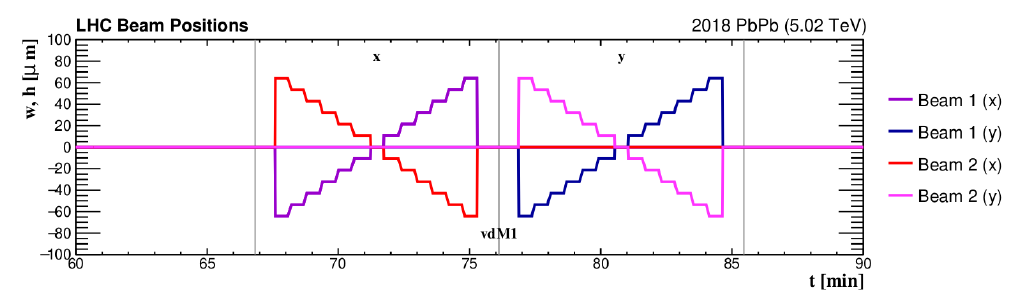
\includegraphics[width=\textwidth]{images/assets/vdm_scan_steps.png}
	\caption{Nominal LHC beam positions displaying the van der Meer scan sequence first in $x$-axis and then in $y$-axis (from \textit{Ref.} \cite{Saariokari:2826125}).}
	\label{fig:vdm_scan_steps}
\end{figure}


% \subsection{Experiment Conditions and Corrective Procedures}

% A vdM scan is conducted under experimental conditions that allow for the measurement of the visible cross-section with the best precision. These conditions include smaller beam intensities, which minimize the effect of MIB and reduce non-linearity effects due to high pileup, well-separated bunches, which minimize afterglow effects where the signal from the previous bunch crossing spills over into the current one, among others \cite{GRAFSTROM201597}. In addition to these optimized experimental conditions, a series of offline corrections are performed to ensure the required level of precision. Such corrections include:

% \begin{itemize}
%     \item Beam current currections: A multitude of different systems measure and monitor the beam conditions during the entire fill in order to allow for offline correction like the removal of non intend charges.
%     \item Background corrections: Background signal, be it beam-induced, detector noise or machine-induced, is typically present in the raw recorded rates. These additional contrinutions are removed.
%     \item Beam Effects: The electromagnetic interaction between the 2 LHC beams results in a disturbance in the nominal beam separation and shapes which effects the calibration measurement. These effects are taken into account and correcti for in the analysis.
%     \item Orbit Drift: During the vdM fill, the nominal position of the LHC beams may shift resulting. These effects are measured by Beam Position Monitors (BPM) that later provide information on how to correct the nominal beam separations.
%     \item Length Scale: The operational displacement of the LHC beams is done with a pair of steering dipoles located on either side of the IP. These displacements come with an associated uncertainty due to effects as magnet hysteresis or lattice imperfection \cite{Persson:2750277}. These uncertainties are also corrected.
%     \item XY Factorization: The vdM method works under the assumption that the tranvese particle distribution are independent in each direction, and therefore factorizable. If this assumption is not true, the calculated value for $A_{eff}$ will be biased. Studies are conducted to understand the magnitude of this bias and correct it.
% \end{itemize}

% A more detailed explanation of these corrections, as well as their impact on the measured calibration, will be given in \autoref{sec:analysis_of_vdm_data}.

\subsection{Experiment Conditions and Corrective Procedures}

A vdM scan is conducted under experimental conditions that allow for the measurement of the visible cross-section with the highest precision. These conditions include smaller beam intensities, which minimize the effect of MIB and reduce non-linearity effects due to high pileup, and well-separated bunches, which minimize afterglow effects where the signal from the previous bunch crossing spills over into the current one, among others \cite{GRAFSTROM201597}. In addition to these optimized experimental conditions, a series of offline corrections are performed to ensure the required level of precision. These corrections include:

\begin{itemize}
    \item \textbf{Beam current corrections:} Various systems measure and monitor the beam conditions throughout the entire fill to enable offline corrections, such as the removal of unintended charges.
    \item \textbf{Background corrections:} Background signals, whether beam-induced, detector noise, or machine-induced, are typically present in the raw recorded rates. These additional contributions are removed.
    \item \textbf{Beam effects:} The electromagnetic interaction between the two LHC beams causes disturbances in the nominal beam separation and shapes, affecting the calibration measurement. These effects are accounted for and corrected in the analysis.
    \item \textbf{Orbit drift:} During the vdM fill, the nominal position of the LHC beams may shift. These shifts are measured by Beam Position Monitors (BPM), which provide information to correct the nominal beam separations.
    \item \textbf{Length scale:} The operational displacement of the LHC beams is achieved using a pair of steering dipoles located on either side of the IP. These displacements come with associated uncertainties due to effects such as magnet hysteresis or lattice imperfections \cite{Persson:2750277}. These uncertainties are corrected.
    \item \textbf{XY factorization:} The vdM method assumes that the transverse particle distributions are independent in each direction and therefore factorizable. If this assumption is not true, the calculated value for \(A_{eff}\) will be biased. Studies are conducted to understand the magnitude of this bias and correct it.
\end{itemize}

A more detailed explanation of these corrections, as well as their impact on the measured calibration, will be provided in \autoref{sec:analysis_of_vdm_data}.


% \subsection{Extrapolation of vdM Calibration}

% The experimental conditions in which a vdM fill is performed, as well as all the extra corrections that are applied to the collected data, ensure a cross-section measurement with high precision and accuracy. However, the experiment conditions that allow for the most optimal probing of the SM, physics conditions, introduce a number of effects that affect the calibration for our luminometers. It is then necessary to extrapolate the results obtained during a vdM fill in order to correctly calibrate the luminosity measured in physics conditions.

% Physics conditions are tailored towards obtaining the largest ammount of data possible. This includes higher bunch populations compared to vdM and more colliding bunches, all of which increase the ammount of colliding particles. These conditions bring about two classes of effects on our luminometers:

% \begin{itemize}
%     \item Efficiency effects: Prolonged exposure to radation in the LHC cavern detiorates the luminometers to the point where they become less efficient. These effects are seen as a decrease in their reported luminosity throughout the data taking year.
%     \item Non linearity effects: The varying experimental conditions can have an effect on the reported luminosity of our detectors, as was already stated in \autoref{subsec:luminosity_detectors}. While some of these effects have their own corrective procedure, like out-of-time pileup \cite{Sirunyan:2759951}, others are corrected empirically.
% \end{itemize}

% In order to account for these 2 classes of effects, the measured luminosity goes through one final correction described by \autoref{eq:luminosity_integration}.

% \begin{equation}
%     \centering
%     \mathcal{L} = \frac{f_{rev} \cdot \mu}{\sigma_{vis} \cdot \epsilon} - \alpha \left( \frac{f_{rev} \cdot \mu}{\sigma_{vis} \cdot \epsilon} \right)^{2}
%     \label{eq:luminosity_integration}
% \end{equation}

% As can be seen, 2 new parameters have been introduced. $\epsilon$ is the parameter that corrects for losses in efficiency in the detector throughout the year. To obtain these factors mini vdM-like scans, called emittance scans, are performed. These scans allow for the measurement of the visible cross-section with the same vdM method, although with less precision, which allows for the analysis of the evolution of this quanity across the year. A figure of merit (FOM) is then calculated as

% \begin{equation}
%     \centering
%     \text{FOM} = \frac{\sigma^{\text{vdM}}_{vis}}{\sigma^{\text{emit}}_{vis}}
%     \label{eq:figure_of_merit}
% \end{equation}

% where $\sigma^{\text{vdM}}_{vis}$ is the visible cross-section measured in vdM conditions and $\sigma^{\text{emit}}_{vis}$ is the one measured in emittance scans during physics conditions. These FOM values are calculated for every emittance scan across the year and are the values given to $\epsilon$ in \autoref{eq:luminosity_integration}. This procedure allows for the extrapolation of the vdM calibration to the rest of the physics fills.

% The second new parameter is $\alpha$ and it is used to correct for any non linearity in the luminometers in an emperical way. Non linearity is defined as any non linear response to changes in the experimental conditions. \autoref{fig:non_linearity_diagram} ilustrates the response of a theoretical linear detector, a detector with positive non linearity and a detector with negative non linearity.

% % \begin{figure}[h]
% % 	\centering
% % 	\includegraphics[width=0.7\textwidth]{images/assets/non_linearity_diagram.pdf}
% % 	\caption{Ilustration of non linearity effects on measured SBIL as a function of the true SBIL. The two marked regions serve the purpose of illustrating the effects of extrapolating from vdM to physics conditions.}
% % 	\label{fig:non_linearity_diagram}
% % \end{figure}

% \begin{figure}[h]
% 	\centering
% 	\makebox[\textwidth][c]{%
% 		\begin{minipage}[b]{0.5\textwidth}
% 			\centering
%             \includegraphics[width=\textwidth]{images/assets/non_linearity_diagram.pdf}
%             \subcaption{}
%             \label{fig:non_linearity_diagram}
% 		\end{minipage}
% 		\begin{minipage}[b]{0.5\textwidth}
% 			\centering
%             \includegraphics[width=\textwidth]{images/assets/non_linearity_method.pdf}
%             \subcaption{}
%             \label{fig:non_linearity_method}
% 		\end{minipage}
% 	}
% 	\caption{(a) Ilustration of non linearity effects on measured SBIL as a function of the true SBIL. The two marked regions serve the purpose of illustrating the effects of extrapolating from vdM to physics conditions. (b) Non linearity extracted for the PLT and BCM1F detectors with respect to DT for fill 9029. Each data point is the ratio of the luminosities averaged over 15 lumi sections.}
% \end{figure}

% The reasons for a detector to have a positive or negative non-linear response differ:

% \begin{itemize}
%     \item PLT has consistently reported signs of suffering from positive non linearity. This mostly comes from the fact that at higher pileup, the probability of a tripple coincidence event occuring accidentally increases, which provoques overcounting.
%     \item HFOC suffers from zero starvation effect and, as explained in \autoref{subsec:zero-counting} this leads to an underestimation of the measured rates which is categorized as a negative non linearity.
%     \item BCM1F, with the VME backend system, has a tendency to undercount at high pileup do to an increasing chance of simultaneous hits being registered as just one hit which lowers the measured rates.
% \end{itemize}

% Correcting for non linearity is challenging due to the lack of a perfectly linear reference detector, which prevents an obsolute measurement of non linearity. Instead, a reference detector, that is assumed to be linear, is used. In this method, a linear fit is performed to the ratio between a luminomter and this reference detector as a function of SBIL. \autoref{fig:non_linearity_method} ilustrates this method applied to PLT and BCM1F while using DT as the reference.

% % \begin{figure}[h]
% %     \centering
% %     \includegraphics[width=0.7\textwidth]{images/assets/non_linearity_method.pdf}
% %     \caption{Non linearity extracted for the PLT and BCM1F detectors with respect to DT for fill 9029. Each data point is the ratio of the luminosities averaged over 15 lumi sections.}
% %     \label{fig:non_linearity_method}
% % \end{figure}

% The slope extracted from the fit is then used as the value of $\alpha$ in \autoref{eq:luminosity_integration}. Unlike the efficiency correctoins, $\epsilon$, the non linearity corrections are done at the expense of introducing some degree of correlation between the corrected detector and the reference. For this reason, and in order to keep the luminometers as independent as possible, the slopes are only extracted for a few fills with high sbil range throughtout the year.


\subsection{Extrapolation of vdM Calibration}

The experimental conditions in which a vdM fill is performed, as well as all the extra corrections applied to the collected data, ensure a cross-section measurement with high precision and accuracy. However, the experimental conditions optimal for probing the Standard Model, known as physics conditions, introduce several effects that impact the calibration of our luminometers. Therefore, it is necessary to extrapolate the results obtained during a vdM fill to correctly calibrate the luminosity measured under physics conditions.

Physics conditions are tailored to obtaining the largest amount of data possible. This includes higher bunch populations compared to vdM fills and more colliding bunches, all of which increase the number of colliding particles. These conditions bring about two classes of effects on our luminometers:

\begin{itemize}
    \item \textbf{Efficiency effects:} Prolonged exposure to radiation in the LHC cavern deteriorates the luminometers, making them less efficient. These effects manifest as a decrease in the reported luminosity throughout the data-taking year.
    \item \textbf{Non-linearity effects:} Varying experimental conditions can affect the reported luminosity of our detectors, as mentioned in \autoref{subsec:luminosity_detectors}. While some of these effects have their own corrective procedures, such as out-of-time pileup \cite{Sirunyan:2759951}, others are corrected empirically.
\end{itemize}

To account for these two classes of effects, the measured luminosity undergoes a final correction described by \autoref{eq:luminosity_integration}.

\begin{equation}
    \centering
    \mathcal{L} = \frac{f_{rev} \cdot \mu}{\sigma_{vis} \cdot \epsilon} - \alpha \left( \frac{f_{rev} \cdot \mu}{\sigma_{vis} \cdot \epsilon} \right)^{2}
    \label{eq:luminosity_integration}
\end{equation}

Two new parameters have been introduced. \(\epsilon\) is the parameter that corrects for losses in detector efficiency throughout the year. To obtain these factors, mini vdM-like scans, called emittance scans, are performed. These scans measure the visible cross-section using the same vdM method, albeit with less precision, allowing for the analysis of the evolution of this quantity over the year. A figure of merit (FOM) is then calculated as:

\begin{equation}
    \centering
    \text{FOM} = \frac{\sigma^{\text{vdM}}_{vis}}{\sigma^{\text{emit}}_{vis}}
    \label{eq:figure_of_merit}
\end{equation}

where \(\sigma^{\text{vdM}}_{vis}\) is the visible cross-section measured under vdM conditions, and \(\sigma^{\text{emit}}_{vis}\) is the one measured during emittance scans under physics conditions. These FOM values are calculated for every emittance scan throughout the year and are assigned to \(\epsilon\) in \autoref{eq:luminosity_integration}. This procedure allows for the extrapolation of the vdM calibration to the rest of the physics fills.

The second new parameter is \(\alpha\), which corrects for any non-linearity in the luminometers empirically. Non-linearity is defined as any non-linear response to changes in experimental conditions. \autoref{fig:non_linearity_diagram} illustrates the response of a theoretical linear detector, a detector with positive non-linearity, and a detector with negative non-linearity.

\begin{figure}[h]
	\centering
	\makebox[\textwidth][c]{%
		\begin{minipage}[b]{0.5\textwidth}
			\centering
            \includegraphics[width=\textwidth]{images/assets/non_linearity_diagram.pdf}
            \subcaption{}
            \label{fig:non_linearity_diagram}
		\end{minipage}
		\begin{minipage}[b]{0.5\textwidth}
			\centering
            \includegraphics[width=\textwidth]{images/assets/non_linearity_method.pdf}
            \subcaption{}
            \label{fig:non_linearity_method}
		\end{minipage}
	}
	\caption{(a) Illustration of non-linearity effects on measured SBIL as a function of the true SBIL. The two marked regions illustrate the effects of extrapolating from vdM to physics conditions. (b) Non-linearity extracted for the PLT and BCM1F detectors with respect to DT for fill 9029. Each data point is the ratio of the luminosities averaged over 15 lumi sections.}
\end{figure}

The reasons for a detector to have a positive or negative non-linear response vary:

\begin{itemize}
    \item PLT has consistently shown signs of positive non-linearity, mainly due to the increased probability of accidental triple coincidence events at higher pileup, leading to overcounting.
    \item HFOC suffers from the zero starvation effect, as explained in \autoref{subsec:zero-counting}, leading to an underestimation of the measured rates, categorized as negative non-linearity.
    \item BCM1F, with the VME backend system, tends to undercount at high pileup due to the increasing chance of simultaneous hits being registered as a single hit, lowering the measured rates.
\end{itemize}

Correcting for non-linearity is challenging due to the lack of a perfectly linear reference detector, which prevents an absolute measurement of non-linearity. Instead, a reference detector assumed to be linear is used. In this method, a linear fit is performed on the ratio between a luminometer and this reference detector as a function of SBIL. \autoref{fig:non_linearity_method} illustrates this method applied to PLT and BCM1F, using DT as the reference.

The slope extracted from the fit is then used as the value of \(\alpha\) in \autoref{eq:luminosity_integration}. Unlike the efficiency corrections (\(\epsilon\)), the non-linearity corrections are done at the expense of introducing some degree of correlation between the corrected detector and the reference. To keep the luminometers as independent as possible, the slopes are extracted for only a few fills with a high SBIL range throughout the year.

\todo{Brief paragraph stating that specialized vdM conditions, the series of corrections we apply to vdm data and the extrapolation to physics conditions all contribute to the challenge of accuratly measuring luminosity at hadron colliders like the LHC.}

% \subsection{Additional scans}

% Other kinds of scans, besides the vdM scan, are also performed at the vdM fill. These other scans are done in order to provide specific insights on the various experimental conditions during the vdM fill:

% \begin{itemize}
%     \item Super Separation scans (ss): These scans are done by maximaly separating the beams in the LHC. This allowsfor an accurate measurement of the brackground signal for each luminometer.
%     \item Beam Imaging scans (bi): In these scans one of the beams is kept fixed in its nominal head on position while the other is scanned. They are used in the beam-imaging method \cite{Klute_2017} that is used in XY factorization analysis. A visible cross-section is also extracted from these scans as it is done to VdM scans.
%     \item Diagonal scans (diag): These scans are vdM scans done at distinct angles. Different variations like +45-45, +30-60 and +60-30 are used to allow the fitting to happen over different regions of the beam overlap. These scans are aslo used in XY factorization studies.
%     \item Offset scans (off): These have the same motion as in vdM scans only one of the beams is not in the nominal head on position. These scans are used in beam shape studies to determine the XY factorization bias.
%     \item Variable/Constant Length Scale scans (vLS, cLS): These scans are used to calibrate the distance by which the steering magnets displace the beams.
% \end{itemize}

% Each scan is separatly recorded and analysed offline. After due analysis, the corrective procedures that have been determined from each of these special scans are applied during the vdM scan analysis in order to correct the extracted detector calibration. In principle, these corrections affect every luminomenter in a similar fashion.

\subsection{Additional Scans}

In addition to the VdM scan, other types of scans are performed during the VdM fill to provide specific insights into the various experimental conditions:

\begin{itemize}
    \item \textbf{Super Separation scans (ss):} These scans involve maximally separating the beams in the LHC, allowing for an accurate measurement of the background signal for each luminometer.
    \item \textbf{Beam Imaging scans (bi):} In these scans, one beam is kept fixed in its nominal head-on position while the other beam is scanned. They are used in the beam-imaging method \cite{Klute_2017}, which is employed in XY factorization analysis. A visible cross-section is also extracted from these scans, similar to VdM scans.
    \item \textbf{Diagonal scans (diag):} These are VdM scans performed at distinct angles, such as +45/-45, +30/-60, and +60/-30. They allow the fitting to occur over different regions of the beam overlap and are used in XY factorization studies.
    \item \textbf{Offset scans (off):} These scans have the same motion as VdM scans, but one of the beams is not in the nominal head-on position. They are used in beam shape studies to determine the XY factorization bias.
    \item \textbf{Variable/Constant Length Scale scans (vLS, cLS):} These scans are used to calibrate the distance by which the steering magnets displace the beams.
\end{itemize}

Each scan is separately recorded and analyzed offline. After thorough analysis, the corrective procedures determined from each of these special scans are applied during the VdM scan analysis to correct the extracted detector calibration. In principle, these corrections affect every luminometer in a similar fashion.
